%%%%%%%%%%%%%%%%%%%%%%%%%%%%%%%%%%%%%%%%%%
% The Legrand Orange Book
% LaTeX Template
% Version 2.4 (26/09/2018)
%
% This template was downloaded from:
% http://www.LaTeXTemplates.com
%
% Original author:
% Mathias Legrand (legrand.mathias@gmail.com) with modifications by:
% Vel (vel@latextemplates.com)
%
% License:
% CC BY-NC-SA 3.0 (http://creativecommons.org/licenses/by-nc-sa/3.0/)
%
% Compiling this template:
% This template uses biber for its bibliography and makeindex for its index.
% When you first open the template, compile it from the command line with the 
% commands below to make sure your LaTeX distribution is configured correctly:
%
% 1) pdflatex main
% 2) makeindex main.idx -s StyleInd.ist
% 3) biber main
% 4) pdflatex main x 2
%
% After this, when you wish to update the bibliography/index use the appropriate
% command above and make sure to compile with pdflatex several times 
% afterwards to propagate your changes to the document.
%
% This template also uses a number of packages which may need to be
% updated to the newest versions for the template to compile. It is strongly
% recommended you update your LaTeX distribution if you have any
% compilation errors.
%
% Important note:
% Chapter heading images should have a 2:1 width:height ratio,
% e.g. 920px width and 460px height.
%
%%%%%%%%%%%%%%%%%%%%%%%%%%%%%%%%%%%%%%%%%

%----------------------------------------------------------------------------------------
%	PACKAGES AND OTHER DOCUMENT CONFIGURATIONS
%----------------------------------------------------------------------------------------

\documentclass[11pt,fleqn]{book} % Default font size and left-justified equations





\usepackage[dvipsnames]{xcolor}






           %%%%%%%%%%%%%%%%%%%%%%%%%%%%%%%%%%%%%%%%%
% The Legrand Orange Book
% Structural Definitions File
% Version 2.1 (26/09/2018)
%
% Original author:
% Mathias Legrand (legrand.mathias@gmail.com) with modifications by:
% Vel (vel@latextemplates.com)
% 
% This file was downloaded from:
% http://www.LaTeXTemplates.com
%
% License:
% CC BY-NC-SA 3.0 (http://creativecommons.org/licenses/by-nc-sa/3.0/)
%
%%%%%%%%%%%%%%%%%%%%%%%%%%%%%%%%%%%%%%%%%

%----------------------------------------------------------------------------------------
%	VARIOUS REQUIRED PACKAGES AND CONFIGURATIONS
%----------------------------------------------------------------------------------------

\usepackage{graphicx} % Required for including pictures
\graphicspath{{Pictures/}} % Specifies the directory where pictures are stored

\usepackage{lipsum} % Inserts dummy text

\usepackage{tikz} % Required for drawing custom shapes

\usepackage[english]{babel} % English language/hyphenation

\usepackage[shortlabels]{enumitem}


% \usepackage{enumitem} % Customize lists
\setlist{nolistsep} % Reduce spacing between bullet points and numbered lists

\usepackage{booktabs} % Required for nicer horizontal rules in tables

\usepackage{xcolor} % Required for specifying colors by name
\definecolor{ocre}{RGB}{243,102,25} % Define the orange color used for highlighting throughout the book
\linespread{1.25}
%----------------------------------------------------------------------------------------
%	MARGINS
%----------------------------------------------------------------------------------------

\usepackage{geometry} % Required for adjusting page dimensions and margins

\geometry{
	paper=a4paper, % Paper size, change to letterpaper for US letter size
	%paper=letterpaper,
	top=3cm, % Top margin
	bottom=3cm, % Bottom margin
	left=3cm, % Left margin
	right=3cm, % Right margin
	headheight=14pt, % Header height
	footskip=1.4cm, % Space from the bottom margin to the baseline of the footer
	headsep=10pt, % Space from the top margin to the baseline of the header
	%showframe, % Uncomment to show how the type block is set on the page
}




\usepackage[normalem]{ulem}
\usepackage{amsmath}
\usepackage[english]{babel}
\usepackage{graphicx}
\usepackage{tabulary}
\usepackage{tabularx}
\usepackage{cancel}
\usepackage{pagecolor}
\usepackage{afterpage}
\usepackage{soul}
\usepackage{fixltx2e}
\usepackage[utf8]{inputenc}
\usepackage{siunitx} %degrees for Laboratory
\usepackage{pdflscape} %sidescape figure in Laboratory
\usepackage{float}
\usepackage{placeins}
\usepackage{afterpage}
\usepackage{xcolor}
\usepackage{framed}
\usepackage{soul}
%\textsubscript{this}
\usepackage{lastpage}
\usepackage[utf8]{inputenc}
\usepackage{ifthen}
\usepackage{amsmath}
\usepackage{fancyhdr}
\usepackage[document]{ragged2e}
% \usepackage[margin=1in,top=1.2in,headheight=57pt,headsep=0.1in]{geometry}
\usepackage{fancyhdr}
\usepackage{caption}
\usepackage{subcaption}
%Chapter 2
\usepackage{rotating}%for sidewaysfigure
\usepackage[final]{pdfpages}
\usepackage{gensymb}
\usepackage[most]{tcolorbox}
%\usepackage[dvipsnames]{xcolor}
\usepackage{colortbl}
\usepackage{chemfig}
\usepackage{lscape}
\usepackage{wrapfig}
\usepackage{float}
% FOR CENTERING TEXT IN TABLE
\usepackage{array}
\usepackage{multirow}
\newcolumntype{C}[1]{>{\centering\arraybackslash}m{#1}}
\usepackage{amsfonts}
\usepackage{amssymb}
\usepackage{mhchem}
\usepackage{stmaryrd}
\usepackage{graphicx}
\usepackage[export]{adjustbox}
\graphicspath{ {./images/} }
\usepackage{makecell}
\usepackage{hyperref}
\usepackage[justification=centering]{caption}
\usepackage{booktabs}% http://ctan.org/pkg/booktabs
\usepackage{wrapfig}
\usepackage{setspace}
\usepackage{pifont}
\usepackage{animate}
\usepackage{imakeidx}
\makeindex\makeindex[columns=3, title=Alphabetical Index, 
           options= -s example_style.ist]
\newcommand{\tabitem}{~~\llap{\textbullet}~~}
\graphicspath{ {./images/} }
%\usetikzlibrary{positioning}
%\usetikzlibrary{decorations.pathreplacing}
%\usetikzlibrary{automata}
%\usetikzlibrary {shapes.multipart}
%\usetikzlibrary{calc}
%\usetikzlibrary{arrows}
%\usetikzlibrary{snakes}
%\usetikzlibrary{calc}
\usetikzlibrary{shapes.multipart, shapes.geometric, arrows}
\usetikzlibrary{calc, decorations.markings}
\usetikzlibrary{arrows.meta}
\usetikzlibrary{shapes,snakes}
\usetikzlibrary{quotes,angles, positioning}
\usetikzlibrary{arrows.meta,
                chains,
                positioning,
                shapes.geometric
                }

\makeatletter
\pgfkeys{/pgf/.cd,
  parallelepiped offset x/.initial=4mm,
  parallelepiped offset y/.initial=4mm
}
\pgfdeclareshape{parallelepiped}
{
  \inheritsavedanchors[from=rectangle] % this is nearly a rectangle
  \inheritanchorborder[from=rectangle]
  \inheritanchor[from=rectangle]{north}
  \inheritanchor[from=rectangle]{north west}
  \inheritanchor[from=rectangle]{north east}
  \inheritanchor[from=rectangle]{center}
  \inheritanchor[from=rectangle]{west}
  \inheritanchor[from=rectangle]{east}
  \inheritanchor[from=rectangle]{mid}
  \inheritanchor[from=rectangle]{mid west}
  \inheritanchor[from=rectangle]{mid east}
  \inheritanchor[from=rectangle]{base}
  \inheritanchor[from=rectangle]{base west}
  \inheritanchor[from=rectangle]{base east}
  \inheritanchor[from=rectangle]{south}
  \inheritanchor[from=rectangle]{south west}
  \inheritanchor[from=rectangle]{south east}
  \backgroundpath{
    % store lower right in xa/ya and upper right in xb/yb
    \southwest \pgf@xa=\pgf@x \pgf@ya=\pgf@y
    \northeast \pgf@xb=\pgf@x \pgf@yb=\pgf@y
    \pgfmathsetlength\pgfutil@tempdima{\pgfkeysvalueof{/pgf/parallelepiped offset x}}
    \pgfmathsetlength\pgfutil@tempdimb{\pgfkeysvalueof{/pgf/parallelepiped offset y}}
    \def\ppd@offset{\pgfpoint{\pgfutil@tempdima}{\pgfutil@tempdimb}}
    \pgfpathmoveto{\pgfqpoint{\pgf@xa}{\pgf@ya}}
    \pgfpathlineto{\pgfqpoint{\pgf@xb}{\pgf@ya}}
    \pgfpathlineto{\pgfqpoint{\pgf@xb}{\pgf@yb}}
    \pgfpathlineto{\pgfqpoint{\pgf@xa}{\pgf@yb}}
    \pgfpathclose
    \pgfpathmoveto{\pgfqpoint{\pgf@xb}{\pgf@ya}}
    \pgfpathlineto{\pgfpointadd{\pgfpoint{\pgf@xb}{\pgf@ya}}{\ppd@offset}}
    \pgfpathlineto{\pgfpointadd{\pgfpoint{\pgf@xb}{\pgf@yb}}{\ppd@offset}}
    \pgfpathlineto{\pgfpointadd{\pgfpoint{\pgf@xa}{\pgf@yb}}{\ppd@offset}}
    \pgfpathlineto{\pgfqpoint{\pgf@xa}{\pgf@yb}}
    \pgfpathmoveto{\pgfqpoint{\pgf@xb}{\pgf@yb}}
    \pgfpathlineto{\pgfpointadd{\pgfpoint{\pgf@xb}{\pgf@yb}}{\ppd@offset}}
  }
}
\makeatother









%Defining colour with different models.
\definecolor{mypink1}{rgb}{0.858, 0.188, 0.478}
\definecolor{mypink2}{RGB}{219, 48, 122}
\definecolor{mypink3}{cmyk}{0, 0.7808, 0.4429, 0.1412}
\definecolor{mygray}{gray}{0.6}
\colorlet{LightRubineRed}{RubineRed!70!}
\colorlet{Mycolor1}{green!10!orange!90!}
\definecolor{Mycolor2}{HTML}{00F9DE}
%\fboxsep=4mm%padding thickness
%\fboxrule=4pt%border thickness

%New command used in the table with all available colour names
\newcommand{\thiscolor}[1]{\texttt{#1} \hfill \fcolorbox{black}{#1}{\hspace{2mm}}}
%----------------------------------------------------------------------------------------
%	FONTS
%----------------------------------------------------------------------------------------

\usepackage{avant} % Use the Avantgarde font for headings
%\usepackage{times} % Use the Times font for headings
\usepackage{mathptmx} % Use the Adobe Times Roman as the default text font together with math symbols from the Sym­bol, Chancery and Com­puter Modern fonts

\usepackage{microtype} % Slightly tweak font spacing for aesthetics
\usepackage[utf8]{inputenc} % Required for including letters with accents
\usepackage[T1]{fontenc} % Use 8-bit encoding that has 256 glyphs

%----------------------------------------------------------------------------------------
%	BIBLIOGRAPHY AND INDEX
%----------------------------------------------------------------------------------------

\usepackage[style=numeric,citestyle=numeric,sorting=nyt,sortcites=true,autopunct=true,babel=hyphen,hyperref=true,abbreviate=false,backref=true,backend=biber]{biblatex}
\addbibresource{bibliography.bib} % BibTeX bibliography file
\defbibheading{bibempty}{}

\usepackage{calc} % For simpler calculation - used for spacing the index letter headings correctly
\usepackage{makeidx} % Required to make an index
\makeindex % Tells LaTeX to create the files required for indexing

%----------------------------------------------------------------------------------------
%	MAIN TABLE OF CONTENTS
%----------------------------------------------------------------------------------------

\usepackage{titletoc} % Required for manipulating the table of contents

\contentsmargin{0cm} % Removes the default margin

% Part text styling (this is mostly taken care of in the PART HEADINGS section of this file)
\titlecontents{part}
	[0cm] % Left indentation
	{\addvspace{5pt}\bfseries} % Spacing and font options for parts
	{}
	{}
	{}

% Chapter text styling
\titlecontents{chapter}
	[1.25cm] % Left indentation
	{\addvspace{12pt}\large\sffamily\bfseries} % Spacing and font options for chapters
	{\color{ocre!60}\contentslabel[\Large\thecontentslabel]{1.25cm}\color{ocre}} % Formatting of numbered sections of this type
	{\color{ocre}} % Formatting of numberless sections of this type
	{\color{ocre!60}\normalsize\;\titlerule*[.5pc]{.}\;\thecontentspage} % Formatting of the filler to the right of the heading and the page number

% Section text styling
\titlecontents{section}
	[1.25cm] % Left indentation
	{\addvspace{3pt}\sffamily\bfseries} % Spacing and font options for sections
	{\contentslabel[\thecontentslabel]{1.25cm}} % Formatting of numbered sections of this type
	{} % Formatting of numberless sections of this type
	{\hfill\color{black}\thecontentspage} % Formatting of the filler to the right of the heading and the page number

% Subsection text styling
\titlecontents{subsection}
	[1.25cm] % Left indentation
	{\addvspace{1pt}\sffamily\small} % Spacing and font options for subsections
	{\contentslabel[\thecontentslabel]{1.25cm}} % Formatting of numbered sections of this type
	{} % Formatting of numberless sections of this type
	{\ \titlerule*[.5pc]{.}\;\thecontentspage} % Formatting of the filler to the right of the heading and the page number

% Figure text styling
\titlecontents{figure}
	[1.25cm] % Left indentation
	{\addvspace{1pt}\sffamily\small} % Spacing and font options for figures
	{\thecontentslabel\hspace*{1em}} % Formatting of numbered sections of this type
	{} % Formatting of numberless sections of this type
	{\ \titlerule*[.5pc]{.}\;\thecontentspage} % Formatting of the filler to the right of the heading and the page number

% Table text styling
\titlecontents{table}
	[1.25cm] % Left indentation
	{\addvspace{1pt}\sffamily\small} % Spacing and font options for tables
	{\thecontentslabel\hspace*{1em}} % Formatting of numbered sections of this type
	{} % Formatting of numberless sections of this type
	{\ \titlerule*[.5pc]{.}\;\thecontentspage} % Formatting of the filler to the right of the heading and the page number

%----------------------------------------------------------------------------------------
%	MINI TABLE OF CONTENTS IN PART HEADS
%----------------------------------------------------------------------------------------

% Chapter text styling
\titlecontents{lchapter}
	[0em] % Left indentation
	{\addvspace{15pt}\large\sffamily\bfseries} % Spacing and font options for chapters
	{\color{ocre}\contentslabel[\Large\thecontentslabel]{1.25cm}\color{ocre}} % Chapter number
	{}  
	{\color{ocre}\normalsize\sffamily\bfseries\;\titlerule*[.5pc]{.}\;\thecontentspage} % Page number

% Section text styling
\titlecontents{lsection}
	[0em] % Left indentation
	{\sffamily\small} % Spacing and font options for sections
	{\contentslabel[\thecontentslabel]{1.25cm}} % Section number
	{}
	{}

% Subsection text styling (note these aren't shown by default, display them by searchings this file for tocdepth and reading the commented text)
\titlecontents{lsubsection}
	[.5em] % Left indentation
	{\sffamily\footnotesize} % Spacing and font options for subsections
	{\contentslabel[\thecontentslabel]{1.25cm}}
	{}
	{}

%----------------------------------------------------------------------------------------
%	HEADERS AND FOOTERS
%----------------------------------------------------------------------------------------

\usepackage{fancyhdr} % Required for header and footer configuration

\pagestyle{fancy} % Enable the custom headers and footers

\renewcommand{\chaptermark}[1]{\markboth{\sffamily\normalsize\bfseries\chaptername\ \thechapter.\ #1}{}} % Styling for the current chapter in the header
\renewcommand{\sectionmark}[1]{\markright{\sffamily\normalsize\thesection\hspace{5pt}#1}{}} % Styling for the current section in the header

\fancyhf{} % Clear default headers and footers
\fancyhead[LE,RO]{\sffamily\normalsize\thepage} % Styling for the page number in the header
\fancyhead[LO]{\rightmark} % Print the nearest section name on the left side of odd pages
\fancyhead[RE]{\leftmark} % Print the current chapter name on the right side of even pages
%\fancyfoot[C]{\thepage} % Uncomment to include a footer

\renewcommand{\headrulewidth}{0.5pt} % Thickness of the rule under the header

\fancypagestyle{plain}{% Style for when a plain pagestyle is specified
	\fancyhead{}\renewcommand{\headrulewidth}{0pt}%
}

% Removes the header from odd empty pages at the end of chapters
\makeatletter
\renewcommand{\cleardoublepage}{
\clearpage\ifodd\c@page\else
\hbox{}
\vspace*{\fill}
\thispagestyle{empty}
\newpage
\fi}

%----------------------------------------------------------------------------------------
%	THEOREM STYLES
%----------------------------------------------------------------------------------------

\usepackage{amsmath,amsfonts,amssymb,amsthm} % For math equations, theorems, symbols, etc

\newcommand{\intoo}[2]{\mathopen{]}#1\,;#2\mathclose{[}}
\newcommand{\ud}{\mathop{\mathrm{{}d}}\mathopen{}}
\newcommand{\intff}[2]{\mathopen{[}#1\,;#2\mathclose{]}}
\renewcommand{\qedsymbol}{$\blacksquare$}
\newtheorem{notation}{Notation}[chapter]

% Boxed/framed environments
\newtheoremstyle{ocrenumbox}% Theorem style name
{0pt}% Space above
{0pt}% Space below
{\normalfont}% Body font
{}% Indent amount
{\small\bf\sffamily\color{ocre}}% Theorem head font
{\;}% Punctuation after theorem head
{0.25em}% Space after theorem head
{\small\sffamily\color{ocre}\thmname{#1}\nobreakspace\thmnumber{\@ifnotempty{#1}{}\@upn{#2}}% Theorem text (e.g. Theorem 2.1)
\thmnote{\nobreakspace\the\thm@notefont\sffamily\bfseries\color{black}---\nobreakspace#3.}} % Optional theorem note

\newtheoremstyle{blacknumex}% Theorem style name
{5pt}% Space above
{5pt}% Space below
{\normalfont}% Body font
{} % Indent amount
{\small\bf\sffamily}% Theorem head font
{\;}% Punctuation after theorem head
{0.25em}% Space after theorem head
{\small\sffamily{\tiny\ensuremath{\blacksquare}}\nobreakspace\thmname{#1}\nobreakspace\thmnumber{\@ifnotempty{#1}{}\@upn{#2}}% Theorem text (e.g. Theorem 2.1)
\thmnote{\nobreakspace\the\thm@notefont\sffamily\bfseries---\nobreakspace#3.}}% Optional theorem note

\newtheoremstyle{blacknumbox} % Theorem style name
{0pt}% Space above
{0pt}% Space below
{\normalfont}% Body font
{}% Indent amount
{\small\bf\sffamily}% Theorem head font
{\;}% Punctuation after theorem head
{0.25em}% Space after theorem head
{\small\sffamily\thmname{#1}\nobreakspace\thmnumber{\@ifnotempty{#1}{}\@upn{#2}}% Theorem text (e.g. Theorem 2.1)
\thmnote{\nobreakspace\the\thm@notefont\sffamily\bfseries---\nobreakspace#3.}}% Optional theorem note

% Non-boxed/non-framed environments
\newtheoremstyle{ocrenum}% Theorem style name
{5pt}% Space above
{5pt}% Space below
{\normalfont}% Body font
{}% Indent amount
{\small\bf\sffamily\color{ocre}}% Theorem head font
{\;}% Punctuation after theorem head
{0.25em}% Space after theorem head
{\small\sffamily\color{ocre}\thmname{#1}\nobreakspace\thmnumber{\@ifnotempty{#1}{}\@upn{#2}}% Theorem text (e.g. Theorem 2.1)
\thmnote{\nobreakspace\the\thm@notefont\sffamily\bfseries\color{black}---\nobreakspace#3.}} % Optional theorem note
\makeatother

% Defines the theorem text style for each type of theorem to one of the three styles above
\newcounter{dummy} 
\numberwithin{dummy}{section}
\theoremstyle{ocrenumbox}
\newtheorem{theoremeT}[dummy]{Theorem}
\newtheorem{problem}{Problem}[chapter]
\newtheorem{exerciseT}{Exercise}[chapter]
\theoremstyle{blacknumex}
\newtheorem{exampleT}{Example}[chapter]
\theoremstyle{blacknumbox}
\newtheorem{vocabulary}{Vocabulary}[chapter]
\newtheorem{definitionT}{Definition}[section]
\newtheorem{corollaryT}[dummy]{Corollary}
\theoremstyle{ocrenum}
\newtheorem{proposition}[dummy]{Proposition}

%----------------------------------------------------------------------------------------
%	DEFINITION OF COLORED BOXES
%----------------------------------------------------------------------------------------

\RequirePackage[framemethod=default]{mdframed} % Required for creating the theorem, definition, exercise and corollary boxes

% Theorem box
\newmdenv[skipabove=7pt,
skipbelow=7pt,
backgroundcolor=black!5,
linecolor=ocre,
innerleftmargin=5pt,
innerrightmargin=5pt,
innertopmargin=5pt,
leftmargin=0cm,
rightmargin=0cm,
innerbottommargin=5pt]{tBox}

% Exercise box	  
\newmdenv[skipabove=7pt,
skipbelow=7pt,
rightline=false,
leftline=true,
topline=false,
bottomline=false,
backgroundcolor=ocre!10,
linecolor=ocre,
innerleftmargin=5pt,
innerrightmargin=5pt,
innertopmargin=5pt,
innerbottommargin=5pt,
leftmargin=0cm,
rightmargin=0cm,
linewidth=4pt]{eBox}	

% Definition box
\newmdenv[skipabove=7pt,
skipbelow=7pt,
rightline=false,
leftline=true,
topline=false,
bottomline=false,
linecolor=ocre,
innerleftmargin=5pt,
innerrightmargin=5pt,
innertopmargin=0pt,
leftmargin=0cm,
rightmargin=0cm,
linewidth=4pt,
innerbottommargin=0pt]{dBox}	

% Corollary box
\newmdenv[skipabove=7pt,
skipbelow=7pt,
rightline=false,
leftline=true,
topline=false,
bottomline=false,
linecolor=gray,
backgroundcolor=black!5,
innerleftmargin=5pt,
innerrightmargin=5pt,
innertopmargin=5pt,
leftmargin=0cm,
rightmargin=0cm,
linewidth=4pt,
innerbottommargin=5pt]{cBox}

% Creates an environment for each type of theorem and assigns it a theorem text style from the "Theorem Styles" section above and a colored box from above
\newenvironment{theorem}{\begin{tBox}\begin{theoremeT}}{\end{theoremeT}\end{tBox}}
\newenvironment{exercise}{\begin{eBox}\begin{exerciseT}}{\hfill{\color{ocre}\tiny\ensuremath{\blacksquare}}\end{exerciseT}\end{eBox}}				  
\newenvironment{definition}{\begin{dBox}\begin{definitionT}}{\end{definitionT}\end{dBox}}	
\newenvironment{example}{\begin{exampleT}}{\hfill{\tiny\ensuremath{\blacksquare}}\end{exampleT}}		
\newenvironment{corollary}{\begin{cBox}\begin{corollaryT}}{\end{corollaryT}\end{cBox}}	

%----------------------------------------------------------------------------------------
%	REMARK ENVIRONMENT
%----------------------------------------------------------------------------------------

\newenvironment{remark}{\par\vspace{10pt}\small % Vertical white space above the remark and smaller font size
\begin{list}{}{
\leftmargin=35pt % Indentation on the left
\rightmargin=25pt}\item\ignorespaces % Indentation on the right
\makebox[-2.5pt]{\begin{tikzpicture}[overlay]
\node[draw=ocre!60,line width=1pt,circle,fill=ocre!25,font=\sffamily\bfseries,inner sep=2pt,outer sep=0pt] at (-15pt,0pt){\textcolor{ocre}{R}};\end{tikzpicture}} % Orange R in a circle
\advance\baselineskip -1pt}{\end{list}\vskip5pt} % Tighter line spacing and white space after remark

%----------------------------------------------------------------------------------------
%	SECTION NUMBERING IN THE MARGIN
%----------------------------------------------------------------------------------------

\makeatletter
\renewcommand{\@seccntformat}[1]{\llap{\textcolor{ocre}{\csname the#1\endcsname}\hspace{1em}}}                    
\renewcommand{\section}{\@startsection{section}{1}{\z@}
{-4ex \@plus -1ex \@minus -.4ex}
{1ex \@plus.2ex }
{\normalfont\large\sffamily\bfseries}}
\renewcommand{\subsection}{\@startsection {subsection}{2}{\z@}
{-3ex \@plus -0.1ex \@minus -.4ex}
{0.5ex \@plus.2ex }
{\normalfont\sffamily\bfseries}}
\renewcommand{\subsubsection}{\@startsection {subsubsection}{3}{\z@}
{-2ex \@plus -0.1ex \@minus -.2ex}
{.2ex \@plus.2ex }
{\normalfont\small\sffamily\bfseries}}                        
\renewcommand\paragraph{\@startsection{paragraph}{4}{\z@}
{-2ex \@plus-.2ex \@minus .2ex}
{.1ex}
{\normalfont\small\sffamily\bfseries}}

%----------------------------------------------------------------------------------------
%	PART HEADINGS
%----------------------------------------------------------------------------------------

% Numbered part in the table of contents
\newcommand{\@mypartnumtocformat}[2]{%
	\setlength\fboxsep{0pt}%
	\noindent\colorbox{ocre!20}{\strut\parbox[c][.7cm]{\ecart}{\color{ocre!70}\Large\sffamily\bfseries\centering#1}}\hskip\esp\colorbox{ocre!40}{\strut\parbox[c][.7cm]{\linewidth-\ecart-\esp}{\Large\sffamily\centering#2}}%
}

% Unnumbered part in the table of contents
\newcommand{\@myparttocformat}[1]{%
	\setlength\fboxsep{0pt}%
	\noindent\colorbox{ocre!40}{\strut\parbox[c][.7cm]{\linewidth}{\Large\sffamily\centering#1}}%
}

\newlength\esp
\setlength\esp{4pt}
\newlength\ecart
\setlength\ecart{1.2cm-\esp}
\newcommand{\thepartimage}{}%
\newcommand{\partimage}[1]{\renewcommand{\thepartimage}{#1}}%
\def\@part[#1]#2{%
\ifnum \c@secnumdepth >-2\relax%
\refstepcounter{part}%
\addcontentsline{toc}{part}{\texorpdfstring{\protect\@mypartnumtocformat{\thepart}{#1}}{\partname~\thepart\ ---\ #1}}
\else%
\addcontentsline{toc}{part}{\texorpdfstring{\protect\@myparttocformat{#1}}{#1}}%
\fi%
\startcontents%
\markboth{}{}%
{\thispagestyle{empty}%
\begin{tikzpicture}[remember picture,overlay]%
\node at (current page.north west){\begin{tikzpicture}[remember picture,overlay]%	
\fill[ocre!20](0cm,0cm) rectangle (\paperwidth,-\paperheight);
\node[anchor=north] at (4cm,-3.25cm){\color{ocre!40}\fontsize{220}{100}\sffamily\bfseries\thepart}; 
\node[anchor=south east] at (\paperwidth-1cm,-\paperheight+1cm){\parbox[t][][t]{8.5cm}{
\printcontents{l}{0}{\setcounter{tocdepth}{1}}% The depth to which the Part mini table of contents displays headings; 0 for chapters only, 1 for chapters and sections and 2 for chapters, sections and subsections
}};
\node[anchor=north east] at (\paperwidth-1.5cm,-3.25cm){\parbox[t][][t]{15cm}{\strut\raggedleft\color{Black}\fontsize{30}{30}\sffamily\bfseries#2}};
\end{tikzpicture}};
\end{tikzpicture}}%
\@endpart}
\def\@spart#1{%
\startcontents%
\phantomsection
{\thispagestyle{empty}%
\begin{tikzpicture}[remember picture,overlay]%
\node at (current page.north west){\begin{tikzpicture}[remember picture,overlay]%	
\fill[ocre!20](0cm,0cm) rectangle (\paperwidth,-\paperheight);
\node[anchor=north east] at (\paperwidth-1.5cm,-3.25cm){\parbox[t][][t]{15cm}{\strut\raggedleft\color{white}\fontsize{30}{30}\sffamily\bfseries#1}};
\end{tikzpicture}};
\end{tikzpicture}}
\addcontentsline{toc}{part}{\texorpdfstring{%
\setlength\fboxsep{0pt}%
\noindent\protect\colorbox{ocre!40}{\strut\protect\parbox[c][.7cm]{\linewidth}{\Large\sffamily\protect\centering #1\quad\mbox{}}}}{#1}}%
\@endpart}
\def\@endpart{\vfil\newpage
\if@twoside
\if@openright
\null
\thispagestyle{empty}%
\newpage
\fi
\fi
\if@tempswa
\twocolumn
\fi}

%----------------------------------------------------------------------------------------
%	CHAPTER HEADINGS
%----------------------------------------------------------------------------------------

% A switch to conditionally include a picture, implemented by Christian Hupfer
\newif\ifusechapterimage
\usechapterimagetrue
\newcommand{\thechapterimage}{}%
\newcommand{\chapterimage}[1]{\ifusechapterimage\renewcommand{\thechapterimage}{#1}\fi}%
\newcommand{\autodot}{.}
\def\@makechapterhead#1{%
{\parindent \z@ \raggedright \normalfont
\ifnum \c@secnumdepth >\m@ne
\if@mainmatter
\begin{tikzpicture}[remember picture,overlay]
\node at (current page.north west)
{\begin{tikzpicture}[remember picture,overlay]
\node[anchor=north west,inner sep=0pt] at (0,0) {\ifusechapterimage\includegraphics[width=\paperwidth]{\thechapterimage}\fi};
\draw[anchor=west] (\Gm@lmargin,-9cm) node [line width=2pt,rounded corners=15pt,draw=ocre,fill=white,fill opacity=0.5,inner sep=15pt]{\strut\makebox[22cm]{}};
\draw[anchor=west] (\Gm@lmargin+.3cm,-9cm) node {\huge\sffamily\bfseries\color{black}\thechapter\autodot~#1\strut};
\end{tikzpicture}};
\end{tikzpicture}
\else
\begin{tikzpicture}[remember picture,overlay]
\node at (current page.north west)
{\begin{tikzpicture}[remember picture,overlay]
\node[anchor=north west,inner sep=0pt] at (0,0) {\ifusechapterimage\includegraphics[width=\paperwidth]{\thechapterimage}\fi};
\draw[anchor=west] (\Gm@lmargin,-9cm) node [line width=2pt,rounded corners=15pt,draw=ocre,fill=white,fill opacity=0.5,inner sep=15pt]{\strut\makebox[22cm]{}};
\draw[anchor=west] (\Gm@lmargin+.3cm,-9cm) node {\huge\sffamily\bfseries\color{black}#1\strut};
\end{tikzpicture}};
\end{tikzpicture}
\fi\fi\par\vspace*{270\p@}}}

%-------------------------------------------

\def\@makeschapterhead#1{%
\begin{tikzpicture}[remember picture,overlay]
\node at (current page.north west)
{\begin{tikzpicture}[remember picture,overlay]
\node[anchor=north west,inner sep=0pt] at (0,0) {\ifusechapterimage\includegraphics[width=\paperwidth]{\thechapterimage}\fi};
\draw[anchor=west] (\Gm@lmargin,-9cm) node [line width=2pt,rounded corners=15pt,draw=ocre,fill=white,fill opacity=0.5,inner sep=15pt]{\strut\makebox[22cm]{}};
\draw[anchor=west] (\Gm@lmargin+.3cm,-9cm) node {\huge\sffamily\bfseries\color{black}#1\strut};
\end{tikzpicture}};
\end{tikzpicture}
\par\vspace*{270\p@}}
\makeatother

%----------------------------------------------------------------------------------------
%	LINKS
%----------------------------------------------------------------------------------------

\usepackage{hyperref}
\hypersetup{hidelinks,backref=true,pagebackref=true,hyperindex=true,colorlinks=false,breaklinks=true,urlcolor=ocre,bookmarks=true,bookmarksopen=false}

\usepackage{bookmark}
\bookmarksetup{
open,
numbered,
addtohook={%
\ifnum\bookmarkget{level}=0 % chapter
\bookmarksetup{bold}%
\fi
\ifnum\bookmarkget{level}=-1 % part
\bookmarksetup{color=ocre,bold}%
\fi
}
}
 % Insert the commands.tex file which contains the majority of the structure behind the template

%\hypersetup{pdftitle={Title},pdfauthor={Author}} % Uncomment and fill out to include PDF metadata for the author and title of the book

%----------------------------------------------------------------------------------------

\begin{document}

%----------------------------------------------------------------------------------------
%	TITLE PAGE
%----------------------------------------------------------------------------------------

\begingroup
\thispagestyle{empty} % Suppress headers and footers on the title page
%\begin{center}
%
\includegraphics[scale=0.6]{Blank.png}\\
%
\includegraphics[scale=0.6]{SCC_Logo_Primary.png}
%\end{center}
%\newpagecolor{Apricot}\afterpage{\restorepagecolor}
\begin{tikzpicture}[remember picture,overlay]
\node[inner sep=0pt] (background) at (current page.center) {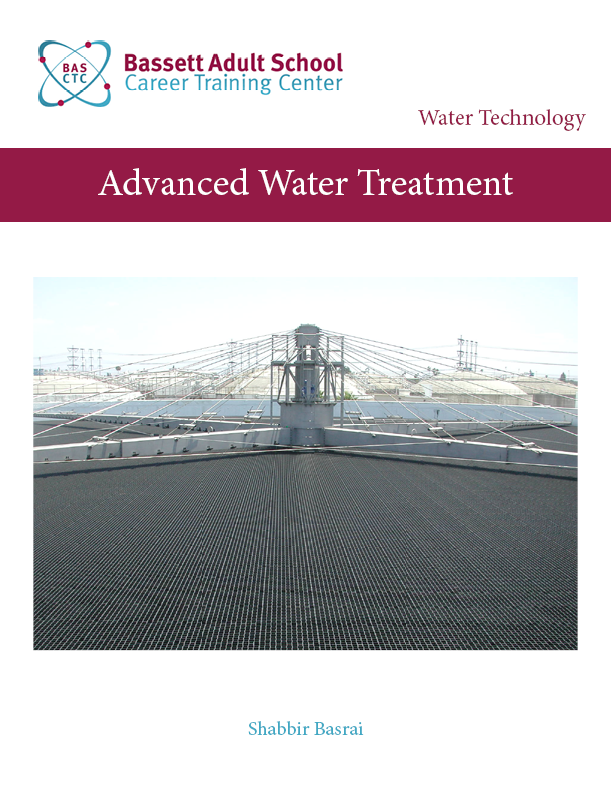
\includegraphics[width=\paperwidth]{BassettCoverAWT}};
%
%\node[inner sep=0pt] (background) at (current page.north east) {
\includegraphics[scale=0.5, angle=-90]{BassettCTCLogo1.png}};
%\node[inner sep=0pt] (background) at (8.1,-1) {
\includegraphics[scale=0.03, angle=0]{waterdrop.jpg}};
%
%\draw (current page.center)node [fill=blue!1!white!10,fill opacity=.003,text opacity=1,inner sep=2cm]at (7,2){ \Huge\centering\bfseries\sffamily\parbox[c][][t]{\paperwidth}{\centering \textcolor{Bittersweet}{} \\\vspace{3cm}\textcolor{BurntOrange}{Drinking Water Treatment \& Distribution}\\[15pt] % Book title
%% {\Large A Profound Subtitle}\\[20pt] % Subtitle
%{}}}; % Author name
\end{tikzpicture}
%\begin{center}
%
\includegraphics[scale=1, angle=-90]{BassettCTCLogo1.png} 
%\end{center}












%\begin{tikzpicture}[]
%\path[help lines,step=.2] (0,0) grid (16,6);
%\path[help lines,line width=.6pt,step=1] (0,0) grid (16,6);
%
%\node[inner sep=0pt] (background) at (current page.center) {\includegraphics[width=\paperwidth]{WaterBackground1.png}};
%\draw (current page.center)node [fill=blue!1!white!10,fill opacity=.3,text opacity=1,inner sep=2cm] { \Huge\centering\bfseries\sffamily\parbox[c][][t]{\paperwidth}{\centering \textcolor{Bittersweet}{October 2022} \\\textcolor{BurntOrange}{Drinking Water Treatment}\\[15pt]
%
%  \pgftext{
\includegraphics[width=300pt, angle =-90]{BassettCTCLogo1.png}} at (16,5);
%%  \pgftext{\includegraphics[width=150pt]{pic2.png}} at (0,0);
%\end{tikzpicture}
\vfill
\endgroup

%----------------------------------------------------------------------------------------
%	COPYRIGHT PAGE
%----------------------------------------------------------------------------------------

\newpage
~\vfill
\thispagestyle{empty}

%\noindent Copyright \copyright\ 2022 Shabbir Basrai\\ % Copyright notice
%
%\noindent \textsc{Published by Publisher}\\ % Publisher
%
%\noindent \textsc{book-website.com}\\ % URL
%
%\noindent Licensed under the Creative Commons Attribution-NonCommercial 3.0 Unported License (the ``License''). You may not use this file except in compliance with the License. You may obtain a copy of the License at \url{http://creativecommons.org/licenses/by-nc/3.0}. Unless required by applicable law or agreed to in writing, software distributed under the License is distributed on an \textsc{``as is'' basis, without warranties or conditions of any kind}, either express or implied. See the License for the specific language governing permissions and limitations under the License.\\ % License information, replace this with your own license (if any)

\noindent \textit{Revision Date: January 2023} % Printing/edition date

%----------------------------------------------------------------------------------------
%	TABLE OF CONTENTS
%----------------------------------------------------------------------------------------

%\usechapterimagefalse % If you don't want to include a chapter image, use this to toggle images off - it can be enabled later with \usechapterimagetrue

\chapterimage{TOCImage} % Table of contents heading image

\pagestyle{empty} % Disable headers and footers for the following pages

\tableofcontents % Print the table of contents itself
\listoffigures
\listoftables
\cleardoublepage % Forces the first chapter to start on an odd page so it's on the right side of the book

\pagestyle{fancy} % Enable headers and footers again

%----------------------------------------------------------------------------------------
%	PART
%----------------------------------------------------------------------------------------



%----------------------------------------------------------------------------------------
%	CHAPTER 1
%----------------------------------------------------------------------------------------

% \chapterimage{chapter_head_2.pdf} % Chapter heading image

% \chapter{Text Chapter}

% \section{Paragraphs of Text}\index{Paragraphs of Text}



% \lipsum[1-7] % Dummy text
% 
%------------------------------------------------

%\section{Citation}\index{Citation}
%
%This statement requires citation \cite{article_key}; this one is more specific \cite[162]{book_key}.

%------------------------------------------------

%\section{Lists}\index{Lists}
%
%Lists are useful to present information in a concise and/or ordered way\footnote{Footnote example...}.
%
%\subsection{Numbered List}\index{Lists!Numbered List}
%
%\begin{enumerate}
%\item The first item
%\item The second item
%\item The third item
%\end{enumerate}
%
%\subsection{Bullet Points}\index{Lists!Bullet Points}
%
%\begin{itemize}
%\item The first item
%\item The second item
%\item The third item
%\end{itemize}
%
%\subsection{Descriptions and Definitions}\index{Lists!Descriptions and Definitions}
%
%\begin{description}
%\item[Name] Description
%\item[Word] Definition
%\item[Comment] Elaboration
%\end{description}1


%----------------------------------------------------------------------------------------
%	PART 2
%----------------------------------------------------------------------------------------


%----------------------------------------------------------------------------------------
%	CHAPTER 1
%----------------------------------------------------------------------------------------

%\chapter{Wastewater Math}
%
\part{Module 1}
\chapterimage{ChapterImageLaboratory.png} % Chapter heading image

\chapter{Background}
\begin{itemize}
\item In the United States, various sources discharge nearly 340 billion gallons of water per day,3 including municipal wastewater, industry process water and cooling water,agriculture runoff and return flows, oil and gas produced wastewater, and stormwater (including rainwater capture).

\item About 322 billion gallons per day is withdrawn in the USA from surface water and ground water sources.

\item While reclaimed water cannot be used to meet all needs, there is great opportunity to increase water reuse to enhance the availability and effective use of water resources.

\item Examples of reuse applications include agricultureand irrigation, potable and non-potable water supplies,groundwater storage and recharge, industrial processes,onsite non-potable use, saltwater intrusion barriers, and environmental restoration.
\end{itemize}

 potable water reuse applications include indirect potable reuse (groundwater replenishment and reservoir water augmentation). 
 
 22 defines the following approved potable uses:
\begin{itemize}
\item Indirect potable reuse (IPR)
\begin{itemize}
\item Groundwater replenishment: the planned use of recycled municipal wastewater that is operated for the purpose of replenishing a groundwater basin designated as a source of municipal and domestic water supply.
\begin{itemize}
\item Surface (spreading) application the application of recharge water to a spreading area for infiltration resulting in the recharge of a groundwater basin or aquifer.
\item Subsurface application the application of recharge water to a groundwater basin(s) by a means other than surface application.
\end{itemize}
\item Reservoir water augmentation: the planned use of recycled municipal wastewater into a surface water reservoir used as a source of domestic drinking water supply.
\end{itemize}
\end{itemize}

\section{Benefits of Water Reuse}
\subsection{Benefits}
Benefits include:
\begin{itemize}
\item improved agricultural production
\item reduced energy consumption associated with production
\item treatment, and distribution of water
\item significant environmental benefits, such as reduced nutrient loads to receiving waters due to reuse of the treated wastewater.
\end{itemize}

\subsection{Drivers}
\begin{itemize}
\item Increases in population and a dependency on high-water-demand agriculture
\item Increasing urbanization; all of these factors and others are effecting 
\item land use changes that exacerbate water supply challenges. 
\item sea level rise and increasing intensity and variability of local climate patterns are predicted to alter hydrologic and ecosystem dynamics and composition
\end{itemize}
Other drivers:
\begin{itemize}
\item Energy efficiency
The water-energy nexus recognizes that water and energy are mutually dependent—energy production requires large volumes of water, and water infrastructure requires large amounts of energy

Water reuse is a critical factor in slowing the compound loop of increased water and energy use witnessed in the water-energy nexus. A frequently-cited definition of sustainability comes from a 1987 report by the Bruntland Commission: “Sustainable development is development that meets the needs of the present without compromising the ability of future generations to meet their own needs” (WCED, 1987). Therefore, sustainable water management can be defined as water resource management that meets the needs of present and future generations.

\end{itemize}
\begin{itemize}
\item increasing need to meet potable water supply demands
\item other urban demands (e.g., landscape irrigation, commercial, and industrial needs)
\item increased agricultural demands due to greater incorporation of animal and dairy products into the diet
\item increase demands on water for food production (Pimentel and Pimentel, 2003). 
\begin{itemize}
\item Potable reuse – Recycled or reclaimed water that is safe for drinking.  There are two types of potable reuse:
\begin{itemize}
\item Indirect Potable Reuse (IPR) - The planned incorporation of reclaimed water into a raw water supply such as in potable water storage reservoirs or a groundwater aquifer, resulting in mixing and assimilation, thus providing an environmental buffer.
\item Direct Potable Reuse (DPR) - The introduction of highly treated reclaimed water either directly into the potable water supply distribution system downstream of a water treatment plant, or into the raw water supply immediately upstream of a water treatment plant.
\end{itemize}
\item While the terms IPR and DPR are still used, there is a transition in terminology to be more specific about the type of potable reuse:
\begin{itemize}
\item Groundwater augmentation (GWA) - Advanced treated water is recharged/injected into the groundwater basin used as a water supply.
\item Surface (reservoir) water augmentation (SWA) - Advanced treated water (+) is discharged into a surface reservoir used as raw water supply. 
\item Raw water augmentation (RWA) - Advanced treated water (++) is discharged directly upstream of a drinking water treatment plant.
\item Treated water augmentation (TWA) - Advanced treated water (+++) is discharged downstream of the drinking water treatment plant directly into the potable water distribution system.
\end{itemize}
\end{itemize}
\end{itemize}
\chapterimage{ChapterImageLaboratory.png} % Chapter heading image

\chapter{Sources and Uses of Recycled Water}

\section{Uses of Recycled Water} \index{Used of Recycled Water}
\begin{enumerate}
\item Irrigation:\\
(a) Recycled water used for the surface irrigation of the following shall be a disinfected tertiary recycled water, except that for filtration pursuant to Section 60301.320(a) coagulation need not be used as part of the treatment process provided that the filter effluent turbidity does not exceed 2 NTU, the turbidity of the influent to the filters is continuously measured, the influent turbidity does not exceed 5 NTU for more than 15 minutes and never exceeds 10 NTU, and that there is the capability to automatically activate chemical addition or divert the wastewater should the filter influent turbidity exceed 5 NTU for more than 15 minutes:
(1) Food crops, including all edible root crops, where the recycled water comes into contact with the edible portion of the crop,
(2) Parks and playgrounds,
(3) School yards,
(4) Residential landscaping,
(5) Unrestricted access golf courses, and
(6) Any other irrigation use not specified in this section and not prohibited by other sections of the California Code of Regulations.
(b) Recycled water used for the surface irrigation of food crops where the edible portion is produced above ground and not contacted by the recycled water shall be at least disinfected secondary-2.2 recycled water.
(c) Recycled water used for the surface irrigation of the following shall be at least disinfected secondary-23 recycled water:
(1) Cemeteries,
(2) Freeway landscaping,
(3) Restricted access golf courses,
(4) Ornamental nursery stock and sod farms where access by the general public is not restricted,
(5) Pasture for animals producing milk for human consumption, and
(6) Any nonedible vegetation where access is controlled so that the irrigated area cannot be used as if it were part of a park, playground or school yard
(d) Recycled wastewater used for the surface irrigation of the following shall be at least undisinfected secondary recycled water:
(1) Orchards where the recycled water does not come into contact with the edible portion of the crop,
(2) Vineyards where the recycled water does not come into contact with the edible portion of the crop,
(3) Non food-bearing trees (Christmas tree farms are included in this category provided no irrigation with recycled water occurs for a period of 14 days prior to harvesting or allowing access by the general public),
(4) Fodder and fiber crops and pasture for animals not producing milk for human consumption,
(5) Seed crops not eaten by humans,
(6) Food crops that must undergo commercial pathogen-destroying processing before being consumed by humans, and
(7) Ornamental nursery stock and sod farms provided no irrigation with recycled water occurs for a period of 14 days prior to harvesting, retail sale, or allowing access by the general public.
(e) No recycled water used for irrigation, or soil that has been irrigated with recycled water, shall come into contact with the edible portion of food crops eaten raw by humans unless the recycled water complies with subsection (a).
\item Impoundments:\\
(a) Except as provided in subsection (b), recycled water used as a source of water supply for nonrestricted recreational impoundments shall be disinfected tertiary recycled water that has been subjected to conventional treatment.
(b) Disinfected tertiary recycled water that has not received conventional treatment may be used for nonrestricted recreational impoundments provided the recycled water is monitored for the presence of pathogenic organisms in accordance with the following:
(1) During the first 12 months of operation and use the recycled water shall be sampled and analyzed monthly for Giardia, enteric viruses, and Cryptosporidium. Following the first 12 months of use, the recycled water shall be sampled and analyzed quarterly for Giardia, enteric viruses, and Cryptosporidium. The ongoing monitoring may be discontinued after the first two years of operation with the approval of the department. This monitoring shall be in addition to the monitoring set forth in section 60321.
(2) The samples shall be taken at a point following disinfection and prior to the point where the recycled water enters the use impoundment. The samples shall be analyzed by an approved laboratory and the results submitted quarterly to the regulatory agency.
(c) The total coliform bacteria concentrations in recycled water used for nonrestricted recreational impoundments, measured at a point between the disinfection process and the point of entry to the use impoundment, shall comply with the criteria specified in section 60301.230 (b) for disinfected tertiary recycled water.
(d) Recycled water used as a source of supply for restricted recreational impoundments and for any publicly accessible impoundments at fish hatcheries shall be at least disinfected secondary-2.2 recycled water.
(e) Recycled water used as a source of supply for landscape impoundments that do not utilize decorative fountains shall be at least disinfected secondary-23 recycled water.

\item Cooling:\\
(a) Recycled water used for industrial or commercial cooling or air conditioning that involves the use of a cooling tower, evaporative condenser, spraying or any mechanism that creates a mist shall be a disinfected tertiary recycled water.
(b) Use of recycled water for industrial or commercial cooling or air conditioning that does not involve the use of a cooling tower, evaporative condenser, spraying, or any mechanism that creates a mist shall be at least disinfected secondary-23 recycled water.
(c) Whenever a cooling system, using recycled water in conjunction with an air conditioning facility, utilizes a cooling tower or otherwise creates a mist that could come into contact with employees or members of the public, the cooling system shall comply with the following:
(1) A drift eliminator shall be used whenever the cooling system is in operation.
(2) A chlorine, or other, biocide shall be used to treat the cooling system recirculating water to minimize the growth of Legionella and other micro-organisms.

\item Other Uses:\\
 Recycled water used for the following shall be disinfected tertiary recycled water, except that for filtration being provided pursuant to Section 60301.320(a) coagulation need not be used as part of the treatment process provided that the filter effluent turbidity does not exceed 2 NTU, the turbidity of the influent to the filters is continuously measured, the influent turbidity does not exceed 5 NTU for more than 15 minutes and never exceeds 10 NTU, and that there is the capability to automatically activate chemical addition or divert the wastewater should the filter influent turbidity exceed 5 NTU for more than 15 minutes:
(1) Flushing toilets and urinals,
(2) Priming drain traps,
(3) Industrial process water that may come into contact with workers,
(4) Structural fire fighting,
(5) Decorative fountains,
(6) Commercial laundries,
(7) Consolidation of backfill around potable water pipelines,
(8) Artificial snow making for commercial outdoor use, and
(9) Commercial car washes, including hand washes if the recycled water is not heated, where the general public is excluded from the washing process.
(b) Recycled water used for the following uses shall be at least disinfected secondary-23 recycled water:
(1) Industrial boiler feed,
(2) Nonstructural fire fighting,
(3) Backfill consolidation around nonpotable piping,
(4) Soil compaction,
(5) Mixing concrete,
(6) Dust control on roads and streets,
(7) Cleaning roads, sidewalks and outdoor work areas and
(8) Industrial process water that will not come into contact with workers.
(c) Recycled water used for flushing sanitary sewers shall be at least undisinfected secondary recycled water.
\end{enumerate}


De facto reuse: A situation where reuse of treated wastewater is, in fact, practiced but is not officially recognized (e.g., a drinking water supply intake located downstream from a wastewater treatment plant [WWTP] discharge point).

Direct potable reuse (DPR): The introduction of reclaimed water (with or without retention in an engineered storage buffer) directly into a drinking water treatment plant, either collocated or remote from the advanced wastewater treatment system.

Indirect potable reuse (IPR): Augmentation of a drinking water source (surface or groundwater) with reclaimed water followed by an environmental buffer that precedes drinking water treatment.

Nonpotable reuse: All water reuse applications that do not involve potable reuse.
Potable reuse: Planned augmentation of a drinking water supply with reclaimed water.

Reclaimed water: Municipal wastewater that has been treated to meet specific water quality criteria with the intent of being used for a range of purposes. The term recycled water is synonymous with reclaimed water.

Water reclamation: The act of treating municipal wastewater to make it acceptable for reuse.
Water reuse: The use of treated municipal wastewater (reclaimed water). Other alternate sources of water, including graywater and stormwater, are discussed in Chapter 2.

Wastewater: Used water discharged from homes, business, industry, and agricultural facilities.
\chapterimage{ChapterImageLaboratory.png} % Chapter heading image

\chapter{Requirements and Regulations}

\section{Title 22 Regulations} \index{Title 22 Regulations}

State of California regulations for how treated and recycled water is used and discharged is listed in Title 22 of the California Administrative Code. The statewide Water Recycling Criteria was developed by the Department of Health Services.  In 2014, the responsibility was transferred to the Division of Drinking Water (DDW) under the California State Water Resources Control Board (SWRCB) and enforced by the nine Regional Water Quality Control Boards (RWQCB).

In the State of California, the California Title 22 Regulations set the requirements to discharge reuse water for different end uses.  By knowing the requirements needed to discharge recycled water, we can identify the necessary treatment processes in order to get there
\chapterimage{ChapterImageLaboratory.png} % Chapter heading image

\chapter{Water Constituents}


\chapterimage{ChapterImageLaboratory.png} % Chapter heading image

\chapter{Treatment Methods}

\section{Ways of Producing Recycled Water} \index{Ways to Produce Recycle Water}

\begin{enumerate}

\item Recycled I - Disinfected Secondary\\

Disinfected secondary effluent can effectively treat COD, BOD, and Pathogens.  However, it does not have a significant impact on any remaining constituents.  This is the lowest level of water reclamation/recycling and has no filtration step.
\begin{itemize}
\item Organics - COD, BOD, TOC
\item Nutrients - TKN, NH3, NO3, NO2, TP, PO4
\item Salts - Na, K, Ca, Mg, Cl, SO4, HCO3
\item Trace Constituents - Boron, Miscellaneous Metals, Hormones, EDCs, PCPs, etc.
\item Pathogens
\end{itemize}

According to Title 22, §60301.225. Disinfected secondary-23 recycled water:\\

"Disinfected secondary-23 recycled water" means recycled water that has been oxidized and disinfected so that the median concentration of total coliform bacteria in the disinfected effluent does not exceed a most probable number (MPN) of 23 per 100 milliliters utilizing the bacteriological results of the last 7 days for which analyses have been completed, and the number of total coliform bacteria does not exceed an MPN of 240 per 100 milliliters in more than one sample in any 30 day period.
 
\item Recycled II - Tertiary with No Nutrient Removal\\

Disinfected tertiary treatment with no nutrient removal can effectively treat COD, BOD, and Pathogens, but does not have a significant impact on the remaining constituents.  This is similar to disinfected secondary.  However, it does have a filtration step, which captures smaller solids particles to reduce turbidity and TSS.  In removing these smaller solids, it may provide better treatment of certain constituents that may be attached or adhered to these solids, such as pathogens.  This is the second lowest level of water reclamation/recycling.
\begin{itemize}
\item Organics - COD, BOD, TOC
\item Nutrients - TKN, NH3, NO3, NO2, TP, PO4
\item Salts - Na, K, Ca, Mg, Cl, SO4, HCO3
\item Trace Constituents - Boron, Miscellaneous Metals, Hormones, EDCs, PCPs, etc.
\item Pathogens
\end{itemize}

Tertiary treatment no nutrient removal with filtration has certain other considerations:
\begin{itemize}
\item Conventional secondary effluent has a relatively low solids retention time (SRT), which essentially translates to smaller floc (clusters of solids) formation.  The smaller the floc, the more difficult it is to filter out the solids; therefore, some solids are more likely pass through the filter.
\item If chlorine is used as the disinfection treatment process, then the ammonia (NH3) can combine with chlorine to form chloramines (NH2Cl, NHCl2), or), which can provide assistance as a disinfectant and can provide longer-lasting disinfection.  
\item However, if the NH3 concentration is low, then there can be challenges with chlorine demand.
\end{itemize}
According to Title 22, §60301.230. Disinfected tertiary recycled water:
\begin{enumerate}
\item The filtered wastewater has been disinfected by either:
\begin{enumerate}
\item A chlorine disinfection process following filtration that provides a CT (the product of total chlorine residual and modal contact time measured at the same point) value of not less than 450 milligram-minutes per liter at all times with a modal contact time of at least 90 minutes, based on peak dry weather design flow; or
\item A disinfection process that, when combined with the filtration process, has been demonstrated to inactivate and/or remove 99.999 percent of the plaque forming units of F-specific bacteriophage MS2, or polio virus in the wastewater.  A virus that is at least as resistant to disinfection as polio virus may be used for purposes of the demonstration.
\end{enumerate}
\item The median concentration of total coliform bacteria measured in the disinfected effluent does not exceed an MPN of 2.2 per 100 milliliters utilizing the bacteriological results of the last seven days for which analyses have been completed and the number of total coliform bacteria does not exceed an MPN of 23 per 100 milliliters in more than one sample in any 30 day period.  No sample shall exceed an MPN of 240 total coliform bacteria per 100 milliliters.
\end{enumerate}
According to Title 22, §60301.320. Filtered wastewater:
"Filtered wastewater" means an oxidized wastewater that meets the criteria in subsection (a) or (b):
\begin{enumerate}
\item Has been coagulated and passed through natural undisturbed soils or a bed of filter media pursuant to the following:
\begin{enumerate}
\item At a rate that does not exceed 5 gallons per minute per square foot of surface area in mono, dual or mixed media gravity, upflow or pressure filtration systems, or does not exceed 2 gallons per minute per square foot of surface area in traveling bridge automatic backwash filters; and
\item So that the turbidity of the filtered wastewater does not exceed any of the following:
\end{enumerate}
\begin{enumerate}
\item An average of 2 NTU within a 24-hour period;
\item 5 NTU more than 5 percent of the time within a 24-hour period; and
\item 10 NTU at any time.
\end{enumerate}
\item Has been passed through a microfiltration, ultrafiltration, nanofiltration, or reverse osmosis membrane so that the turbidity of the filtered wastewater does not exceed any of the following:
\begin{enumerate}
\item 0.2 NTU more than 5 percent of the time within a 24-hour period; and
\item 0.5 NTU at any time.
\end{enumerate}
\end{enumerate}

\item Recycled III - Tertiary with Nutrient Removal\\

Disinfected tertiary treatment with nutrient removal can effectively treat the same constituents as the previous types of recycled water (COD, BOD, and Pathogens), but it also treats nutrients (TKN, NH3, NO3, NO2)!  Other remaining constituents are not significantly impacted.
\begin{itemize}
\item Organics - COD, BOD, TOC
\item Nutrients - TKN, NH3, NO3, NO2, TP, PO4
\item Salts - Na, K, Ca, Mg, Cl, SO4, HCO3
\item Trace Constituents - Boron, Miscellaneous Metals, Hormones, EDCs, PCPs, etc.
\item Pathogens
\end{itemize}

Note that in the wastewater treatment industry, the term "nutrient removal" is often used even when only talking about nitrogen removal  (TKN, NH3, NO3, NO2) and does not generally include phosphorus (TP, PO4).  This is primarily because it is relatively common for treatment plants to have effluent nitrogen limits, but not phosphorus limits.  High levels of nitrogen or phosphorus can potentially cause issues to the receiving water body.  Many water agencies closely follow developing rules and regulations to anticipate the likelihood of receiving stricter nutrient (N or P) limits in their NPDES/WDR permits from the RWQCB.  If a facility does remove nitrogen and phosphorus, then it is often referred to as "nutrient removal and phosphorus removal" or "enhanced biological phosphorus removal (EBPR)."

In 2002, the Elsinore Valley Municipal Water District (EVMWD) received a permit to discharge recycled water from its Regional Wastewater Treatment Plant into Lake Elsinore as part of a 2-year pilot project to research the effects of recycled water.  Lake Elsinore is a natural recreational lake and is subject to high losses due to evaporation (about 14,000 AFY).  The permit required the recycled water to meet a total nitrogen (TN) limit of 3 mg/L and total phosphorus (TP) limit of 0.5 mg/L.  About 2,000 AF of recycled water was discharged into Lake Elsinore for the remaining six months of 2002.  This is the first time that recycled water was released into a recreational lake in California!  This practice continues on today!  
 
\item Recycled IV - Tertiary with Ultrafiltration (UF) or Microfiltration (MF) and Nutrient Removal\\

Disinfected tertiary treatment with ultrafiltration (UF) or microfiltration (MF) membranes and nutrient removal can effectively treat the same constituents as the previous types of recycled water (COD, BOD, Pathogens, TKN, NH3, NO3, NO2) and to a much improved water quality.  This is because previous types of recycled water referred to filtration, which is often a type of monomedia or dual media consisting of sand and/or anthracite (i.e. coal) or a cloth media filter.  While this does provide effective filtration, it is typically in the particulate filtration range to capture particle sizes of 1 micron (micrometer or µm) or larger.  Additionally, channels can develop in media filters whereby allowing even larger particle sizes to pass through. UF or MF refers to filtration via membranes, which have a more consistent pore size (0.01 to 0.1 µm) that limits the size of particles that can pass through the filter.  By removing smaller solids particles via UF or MF membranes, the water quality produced is significantly improved and disinfection efficiency is increased to remove more pathogens.  Other remaining constituents (salts and trace) are not significantly impacted.
\begin{itemize}
\item Organics - COD, BOD, TOC
\item Nutrients - TKN, NH3, NO3, NO2, TP, PO4
\item Salts - Na, K, Ca, Mg, Cl, SO4, HCO3
\item Trace Constituents - Boron, Miscellaneous Metals, Hormones, EDCs, PCPs, etc.
\item Pathogens
\end{itemize}

This type of recycled water is generally produced from more advanced treatment technologies, such as a membrane bioreactor (MBR).  MBR uses both biological processes and membrane technology to treat and filter water.  Organic matter (and potentially nutrients) are removed using biological treatment processes, then membranes filter out the microscopic particles and microorganisms to produce permeate (i.e. water that permeated through the membrane) for downstream disinfection.
 
\item Recycled V - Tertiary with Advanced Oxidation Process (AOP)\\

Disinfected tertiary treatment with advanced oxidation processes (AOP) can effectively treat the same constituents as the previous types of recycled water (COD, BOD, Pathogens, TKN, NH3, NO3, NO2) and it can also treat potentially harmful dissolved organics (TOC) and some trace constituents (boron, miscellaneous metals, hormones, EDCs, PCPs, etc.).  Trace constituents are somewhat difficult to treat considering that they are in the parts per billion (µg/L) range as opposed to typical conventional constituents that are in the parts per million (mg/L) range.
  
\begin{itemize}
\item Organics - COD, BOD, TOC
\item Nutrients - TKN, NH3, NO3, NO2, TP, PO4
\item Salts - Na, K, Ca, Mg, Cl, SO4, HCO3
\item Trace Constituents - Boron, Miscellaneous Metals, Hormones, EDCs, PCPs, etc.
\item Pathogens
\end{itemize}

AOP treats trace constituents by introducing or generating a strong oxidant into the flow that will break down (i.e., break apart) chemicals and dissolved organic material so they are no longer harmful and disinfect water.  Biological Activated Carbon (BAC) filters can in conjunction with AOP to remove dissolved organic material whereby organics stick to the filter and beneficial bacteria, which thrive in a high oxygen environment and live on the filters, eat the organics.
 
\item Recycled VI - Tertiary with AOP and Desalination\\

Disinfected tertiary treatment with AOP and desalination is the highest level of treatment and can effectively treat all typical constituents found in wastewater. 
\begin{itemize}
\item Organics - COD, BOD, TOC
\item Nutrients - TKN, NH3, NO3, NO2, TP, PO4
\item Salts - Na, K, Ca, Mg, Cl, SO4, HCO3
\item Trace Constituents - Boron, Miscellaneous Metals, Hormones, EDCs, PCPs, etc.
\item Pathogens
\end{itemize}

The Orange County Water District (OCWD), West Basin Municipal Water District (WBMWD), and Water Replenishment District (WRD) are a few local Southern California water agencies that produce this type of advanced treated recycled water for groundwater augmentation (GWA) (which is also called groundwater replenishment or groundwater recharge) and/or seawater intrusion barrier.  This water can either be applied to surface recharge basins or injected into the groundwater aquifer via injection wells.

The advanced treatment process at OCWD's Groundwater Replenishment System (GWRS) includes MF, RO, AOP, UV, and mineral stabilization.  Later on in the course, we'll take virtual tour of their treatment process and how they use the advanced treated water, which is actually cleaner than your drinking water! 



\end{enumerate}
\chapterimage{ChapterImageLaboratory.png} % Chapter heading image

\chapter{Recycled Water Distribution}


\section{Recycled Water General Requirements} \index{Recycle Water General Requirements}
\subsection{Recycled Water Use Constraints} \index{Recycle Water Use Constraints}
(a) No irrigation with disinfected tertiary recycled water shall take place within 50 feet of any domestic water supply well unless all of the following conditions have been met:
(1) A geological investigation demonstrates that an aquitard exists at the well between the uppermost aquifer being drawn from and the ground surface.
(2) The well contains an annular seal that extends from the surface into the aquitard.
(3) The well is housed to prevent any recycled water spray from coming into contact with the wellhead facilities.
(4) The ground surface immediately around the wellhead is contoured to allow surface water to drain away from the well.
(5) The owner of the well approves of the elimination of the buffer zone requirement.
(b) No impoundment of disinfected tertiary recycled water shall occur within 100 feet of any domestic water supply well.
(c) No irrigation with, or impoundment of, disinfected secondary-2.2 or disinfected secondary-23 recycled water shall take place within 100 feet of any domestic water supply well.
(d) No irrigation with, or impoundment of, undisinfected secondary recycled water shall take place within 150 feet of any domestic water supply well.
(e) Any use of recycled water shall comply with the following:
(1) Any irrigation runoff shall be confined to the recycled water use area, unless the runoff does not pose a public health threat and is authorized by the regulatory agency.
(2) Spray, mist, or runoff shall not enter dwellings, designated outdoor eating areas, or food handling facilities.
(3) Drinking water fountains shall be protected against contact with recycled water spray, mist, or runoff.
(f) No spray irrigation of any recycled water, other than disinfected tertiary recycled water, shall take place within 100 feet of a residence or a place where public exposure could be similar to that of a park, playground, or school yard.
(g) All use areas where recycled water is used that are accessible to the public shall be posted with signs that are visible to the public, in a size no less than 4 inches high by 8 inches wide, that include the following wording: “RECYCLED WATER - DO NOT DRINK”. Each sign shall display an international symbol similar to that shown in figure 60310-A. The Department may accept alternative signage and wording, or an educational program, provided the applicant demonstrates to the Department that the alternative approach will assure an equivalent degree of public notification.
(h) Except as allowed under section 7604 of title 17, California Code of Regulations, no physical connection shall be made or allowed to exist between any recycled water system and any separate system conveying potable water.
(i) Except for use in a cemetery that complies with the requirements of section 8118 of the Health and Safety Code, the portions of the recycled water piping system that are in areas subject to access by the general public shall not include any hose bibs. Only quick couplers that differ from those used on the potable water system shall be used on the portions of the recycled water piping system in areas subject to public access.
Credits

\subsection{Recycled Water Dual Water System Delivery} \index{Recycle Water Dual Water System Delivery}
No person other than a recycled water agency shall deliver recycled water to a dual-plumbed facility.
(b) Except as allowed pursuant to section 13553(d) of the Water Code, a recycled water agency shall not deliver recycled water for any internal use to any individually-owned residential units including free-standing structures, multiplexes, or condominiums.
(c) No recycled water agency shall deliver recycled water for internal use except for fire suppression systems, to any facility that produces or processes food products or beverages. For purposes of this Subsection, cafeterias or snack bars in a facility whose primary function does not involve the production or processing of foods or beverages are not considered facilities that produce or process foods or beverages.
(d) No recycled water agency shall deliver recycled water to a facility using a dual plumbed system unless the report required pursuant to section 13522.5 of the Water Code, and which meets the requirements set forth in section 60314, has been submitted to, and approved by, the regulatory agency.
Credits

\subsection{Recycled Water Dual Water System Design Requirements} \index{Recycle Water Dual Water System Design Requirements}

The public water supply shall not be used as a backup or supplemental source of water for a dual-plumbed recycled water system unless the connection between the two systems is protected by an air gap separation which complies with the requirements of sections 7602(a) and 7603(a) of title 17, California Code of Regulations, and the approval of the public water system has been obtained.


\subsection{Recycled Water Dual Water System Operation Requirements} \index{Recycle Water Dual Water System Operation Requirements}
(a) Prior to the initial operation of the dual-plumbed recycled water system and annually thereafter, the Recycled Water Agency shall ensure that the dual plumbed system within each facility and use area is inspected for possible cross connections with the potable water system. The recycled water system shall also be tested for possible cross connections at least once every four years. The testing shall be conducted in accordance with the method described in the report submitted pursuant to section 60314. The inspections and the testing shall be performed by a cross connection control specialist certified by the California-Nevada section of the American Water Works Association or an organization with equivalent certification requirements. A written report documenting the result of the inspection or testing for the prior year shall be submitted to the department within 30 days following completion of the inspection or testing.
(b) The recycled water agency shall notify the department of any incidence of backflow from the dual-plumbed recycled water system into the potable water system within 24 hours of the discovery of the incident.
(c) Any backflow prevention device installed to protect the public water system serving the dual-plumbed recycled water system shall be inspected and maintained in accordance with section 7605 of Title 17, California Code of Regulations.


\end{document}
